In this chapter, we describe the implementation details to create the dynamic benchmark DyPyBench based on our approach.
We use various tools and libraries to accomplish the goals of ready-to-run, ready-to-analyze, versatile, extensible, diverse and large-scale for our benchmark.
In the following sections, we describe the concrete steps we perform for implementation and the tools and libraries we use.
The source code of this implementation is present on GitHub at \url{https://github.com/sola-st/master-thesis-piyush-bajaj/tree/automation}.

\begin{figure}[ht]
    \centering
    
\includegraphics[width=1\linewidth]{figures/implementation/implementaion_flow.png}
    \caption{Implementation Flow}
    \label{fig:implementation_flow}
\end{figure}

Figure \ref{fig:implementation_flow} shows the flow of implementation steps for the creation of DyPyBench. 
We start with installation and setup of sample projects from the awesome-python corpus (Section \ref{impl:Sample Projects}).
With these sample projects, we create an automation script to gather a list of 50 Python projects for our benchmark (Section \ref{impl:Automation for Installation}).
We then create a Docker image for our benchmark, and use the list of projects to install and setup the execution environment automatically (Section \ref{impl:Docker Image}).
With the Docker environment ready with the projects, we create a command-line access interface to the benchmark (Section \ref{impl:Access Interface}).   
We integrate LExecutor, PyCG and DynaPyt to the benchmark and provide options for their usage through the access interface (Section \ref{impl:Integrating Tools}).
Finally, we implement Call Graph Analysis in DynaPyt to generate run-time call graphs (Section \ref{impl:Call Graph Analysis}).

\section{Sample Projects}
\label{impl:Sample Projects}
As mentioned in the approach, we select the projects belonging to the different application domains from a predefined set of 679 projects from the the awesome-python project.
We use the table of contents as the application domain for selection.
Figure \ref{fig:awesome-python-website} shows the awesome-python website with the table of contents and some projects.
Source code of these projects is fetched from GitHub repository which is provided by awesome-python or project website linked by awesome-python.  
\begin{figure}
    \centering
    \includegraphics[width=1\linewidth, height=1\linewidth]{figures/implementation/Awesome-Python-website3.png}
    \caption{Awesome Python Website}
    \label{fig:awesome-python-website}
\end{figure}

We decide to select 5 sample projects to start our implementation.
We start by manually picking a random project from one of the categories in the awesome-python corpus.
Then the number of stars for the project repository on GitHub is checked.
If the project has less than 500 stars we choose another project randomly, otherwise we proceed with the picked project.
This helps us to ensure the GitHub stars selection criteria mentioned in section \ref{approach:selection criteria}.
We proceed by cloning the source code of the project and installing it in a Python virtual environment.
If the project is successfully installed, we add the pytest library to the virtual environment.
Finally, the test suite of the project is run using pytest. 
The project is chosen only if the execution is successful ensuring the selection criteria of presence and execution of test suite.

All the above steps are repeated a number of times to get 5 different projects.
Each time a random project is selected, we ensure that it does not belong to a category which has been chosen before.
This helps us fulfill the selection criteria of diverse domain mentioned in section \ref{approach:selection criteria}.
Table \ref{table:first_5_projects} shows a list the projects which were chosen for installation till 5 of them satisfied all the selection criteria.
The 5 projects with \textbf{Yes} in the Criteria column were chosen as the sample projects for further tasks for our benchmark.
We installed some operating system libraries and module dependencies for some of the projects listed in Table \ref{table:first_5_projects} for them to work properly.  

\begin{table}[ht]
    \centering
    \begin{tabular}{lllll}
    \hline
    \textbf{Category} & \textbf{Sub-category} & \textbf{Name} & \textbf{GitHub Stars} & \textbf{Criteria}\\
    \hline
    Web Crawling & - & grab & 2.2k & Yes\\
    DevOps Tools & SSH-style Deployment & fabric & 13.7k & No\\
    Robotics & - & PythonRobotics & 16.8k & Yes\\
    RESTful API & Flask & flask-api & 1.3k & Yes\\
    Deep Learning & - & mxnet & 20.2k & No\\
    Machine Learning & - & gym & 29k & No\\
    Job Scheduler & - & schedule & 10.2k & Yes\\
    Image processing & - & pagan & 278 & No\\
    Image Processing & - & pillow & 10.3k & Yes\\
    \hline
    \end{tabular}
    \caption{First 5 Projects for DyPyBench (Criteria : Test Suite Execution)}
    \label{table:first_5_projects}
\end{table}

\section{Automation for Installation}
\label{impl:Automation for Installation}
The installation and setup of the 5 sample projects helped us in understanding the general steps required for installing 50 steps.
Although, it is possible to install all the 50 projects manually, however, we need to ensure our selection criteria are met.
To do so, we might need to perform the installation of much more projects than 50.
In order to make it easier and quicker to get the list of 50 projects which satisfy our needs, we automate the process of installation and execution of projects.
We use bash scripts for this since they support loops such as while for repetition and conditional statements such as if then else for exceptions.

In order to create the bash script, we use the steps performed in sample projects. 
The Figure \ref{fig:setup difference} shows the installation steps for two sample projects we installed before.
The blue colored text indicates similarities, whereas the red colored text indicates the differences.
\begin{figure}[ht]
    \centering
    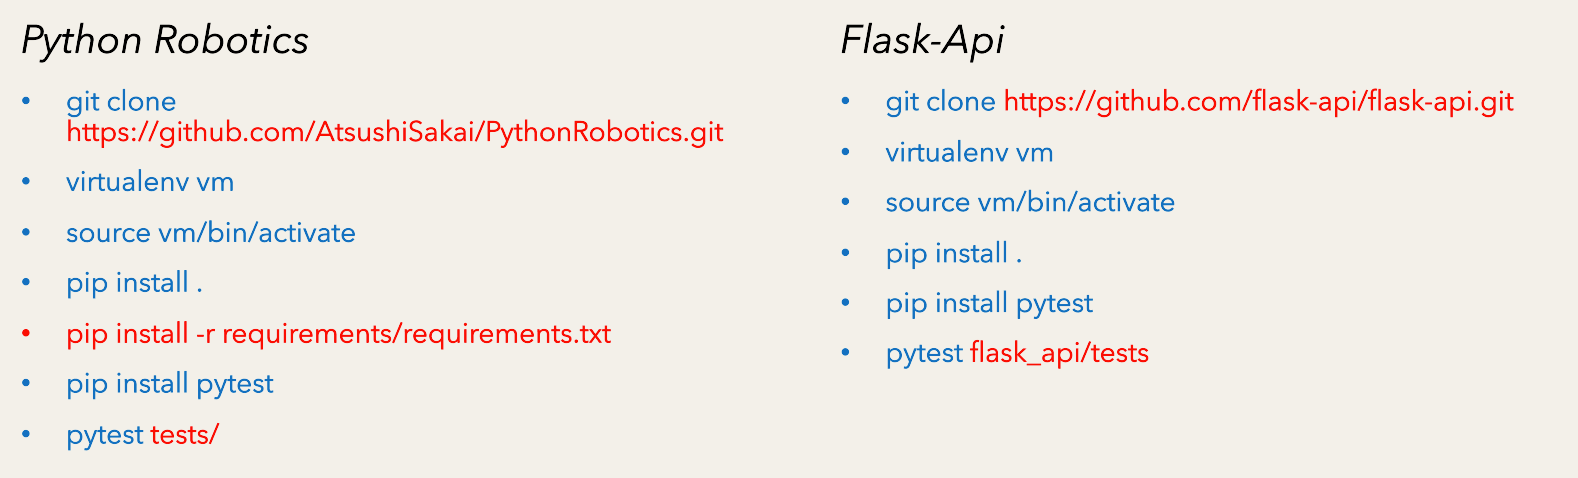
\includegraphics[width=1\linewidth]{figures/implementation/Setup-difference.png}
    \caption{Execution of Projects (Similarities and Differences)}
    \label{fig:setup difference}
\end{figure}
As can be seen from the Figure \ref{fig:setup difference}, the two commands of git clone and pytest have different arguments depending on the project.
Furthermore, the project Python Robotics executes an extra command of pip install, since this project provides us with a requirements.txt file.
A bash script can accept command-line arguments and use these to execute different commands or same command with different arguments.
In this work, instead of the command-line arguments we use a text file to provide these arguments to the bash script.
We create a github-url.txt file, which contains the arguments that the bash script needs.
Each line in github-url.txt contains the arguments for one project.
The Listing \ref{code:github-url-2} shows the entry of two projects shown in the Figure \ref{fig:setup difference} in github-url.txt file.
\lstset{numbers=left, numberstyle=\tiny, stepnumber=1, numbersep=5pt, columns=flexible, breaklines=true}
\lstset{basicstyle=\ttfamily}
\lstset{frame=tb}
\begin{lstlisting}[float,caption=Sample Entry github-url.txt,label=code:github-url-2,language=Bash]
https://github.com/AtsushiSakai/PythonRobotics.git rt requirements/requirements.txt tests
https://github.com/flask-api/flask-api.git t flask_api/tests
\end{lstlisting}

As seen in the Listing \ref{code:github-url-2}, each line contains a collection of space separated strings.
The first line contains 4 strings in total whereas the second line contains only 3.
The first string on both lines is the Git URL of the repository to clone and caters to the difference in the git clone command.
The last string on both lines, i.e., 4th on line 1 and 3rd on ĺine 2, is the test directory path from the project root and caters to the pytest command.
The second string on both lines represents a flag wot indicate the presence or absence of the requirements file.
The possible values for the flag are \textit{rt} or \textit{t}, where the first specifies the presence and second specifies the absence.
If the requirement file is present then we specify the path to the requirement file from the project root, as done in line 1 as a third string in the collection. 
This string caters the difference of the extra \textbf{pip install} command described above. 

The automation script we create, starts by creating a Project directory if it does not exists.
Then we read the github-url.txt file we created before line by line and perform the following steps for each line.
First, we split the space separated strings to get the arguments as described before.
We then create a numbered sub-folder for the project to be installed and clone the source code from the Git URL into the sub-folder.
Inside the sub-folder, we create a Python virtual environment \textit{.vm} and activate this environment.
We then install the project using the source code.
Next, we check if the flag provided is \textit{rt}, if yes, then we install the dependencies using the requirements file.
We then check, if the the project needs some extra dependencies to execute test suite and install those if needed.
This check is based on the Git URL of the project.
We proceed by installing the pytest library to the virtual environment.
Finally, we execute the test suite using pytest.
The automation bash script we create for installation and execution to gather a list 50 projects is provided in Listing \ref{code:project_selection_automation.sh}.

With the sample projects, we get 5 entries in github-url.txt.
The next step is to include more projects in this list.
For this, we start by picking random projects from awesome-python and check for GitHub stars selection criteria.
If the criteria is met, we add an entry to github-url.txt file as per the format.
We add 10 such entries at a time and run the automation script we created before.
If the installation and execution was successful, we then select the project for our list.
We try to fix issues related to module dependency, if they occur and rerun the test suite for some projects.
If needed, we modify the automation script to install these dependencies during installation. 
We repeat the steps of adding 10 projects until we have 50 projects which install and execute properly.
The list of the 50 projects that we use in DyPyBench is provided in \ref{table:50_installed_projects}.

\section{Docker Image}
\label{impl:Docker Image}
With the list of projects and the automation script, we can install and setup our projects for use.
Since we package our benchmark as a Docker image, we create one and install our projects in it.
We use Ubuntu as the base image, since we performed the previous steps in our implementation on a Ubuntu machine and have the list of system dependencies we would need.
Also, we created bash files which can only run on Linux based systems.
We first create a simple image for the benchmark with the required system dependencies and the source code files of DyPyBench.
This image is created using the Dockerfile provided in Listing \ref{code:Dockerfile}.
\begin{lstlisting}[caption=Dockerfile,label=code:Dockerfile,language=Bash]
FROM ubuntu:latest

WORKDIR /DyPyBench

RUN apt-get update

RUN apt-get install python3 -yq

RUN apt install python3-pip -yq

RUN apt install python3-virtualenv -yq

RUN apt install git -yq

RUN apt install nano -yq

RUN apt install libjpeg8-dev -yq

RUN apt-get install ffmpeg libavcodec-extra -yq

RUN pip install --upgrade pip setuptools wheel

COPY . .

RUN chmod -R 777 ./scripts 
\end{lstlisting}

We can see from the Listing \ref{code:Dockerfile}, we install git, nano, python3, python3-pip and python3-virtualenv to our image.
We also install libjpeg8-dev, ffmpeg and libavcodec-extra as these are needed by Pillow and pydub projects.
After copying the source files into the working directory of \textit{/DyPyBench} on line 23, we modify the permissions of the scripts folder to allow execution of bash scripts.

The Docker image created so far contains the source files for DyPyBench, automation scripts and the list of projects in the github-url.txt.
We create a container from this image and run a bash script to automatically install and setup the projects from the list.
This script performs the same steps as provided by the automation script in Listing \ref{code:project_selection_automation.sh} except for two steps.
First is the non execution of the test suite and second is the overwriting of test files.
Test suite execution is not needed since we in this step we are providing the selected projects for the benchmark and test execution was a selection criteria.
We overwrite test files to skip the failed test cases for analysis frameworks to work efficiently. 
After installing the projects from the list, we create the image from this container and export it on Docker Hub where the image name is dypybench/dypybench and the tag is v1.0.
Figure \ref{fig:dypybench docker} shows the created image on the Docker Hub website \footnote{https://hub.docker.com/}, available as a public repository.

\begin{figure}[ht]
\centering
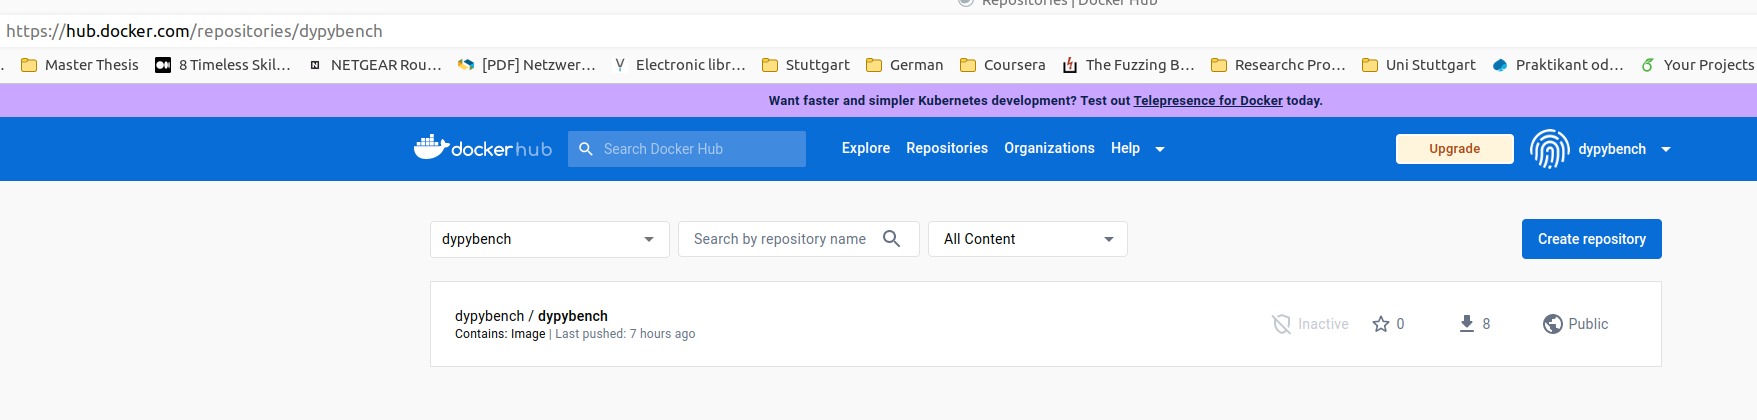
\includegraphics[width=1\linewidth]{figures/implementation/docker_hub.png}
\caption[DyPyBench Docker Hub]{\label{fig:dypybench docker}Docker Hub}
\end{figure}

\section{Access Interface}
\label{impl:Access Interface}
In order to allow easy access to the collection of projects in the Docker image, we create a single command-line interface with Python script.
Python scripts are user-friendly and offer extensive support for both standard and third-party libraries that can be utilized for automating tasks, data processing, and analysis.
They are also easily extensible, allowing for the addition of new features without affecting the previous functionality.
These scripts can be triggered from the command-line and also accept command line options.

In this work, we create a Python script, dypybench.py, which acts as a single point of entry to trigger the execution of various tasks within the benchmark.
The script is executed from the command-line using the command as shown below.

\verb$python3 dypybench.py <args>$

The command-line arguments to the script are parsed with the standard Python library of argparse.
The script first reads the github-url.txt file and stores some information related to the projects.
The information stored is the mapping from project number to name and the collection of strings arguments as described earlier in section \ref{impl:Automation for Installation}.
The initial command-line arguments added to the script are \textit{\--\--list}, \textit{\--\--save}, \textit{\--\--test}, \textit{\--\--test\_original} and \textit{\--\--timeout}.
The argument \textit{\--\--list}, prints the number, name and Git URL of all the projects in the benchmark.
The argument \textit{\--\--save}, copies the output to the file specified.
The argument \textit{\--\--test}, executes the test suite of the project number specified to this argument.
Essentially, the Python script triggers a new process using the subprocess module to execute the bash script provided to run the test suite with the arguments provided in github-url.txt.
The argument \textit{\--\--test\_original} can be combined with \textit{\--\--test} and specifies the tests to be performed on the original copy of the code.  
Lastly, the argument \textit{\--\--timeout}, kills the subprocess and any command from the bash script that is still running after the seconds specified to this argument.  
More arguments are added to this interface when we add the analysis frameworks and LExecutor.
Each of those arguments executes a new process to execute a specific bash script.
These arguments are explained in their respective sections later.
Multiple projects can be specified by space separated numbers in the respective arguments, whereas the project number 0 specifies the task to be run on all the 50 projects.  
In order to avoid manipulation to the source code, we create a duplicate copy of the project specified and perform the task on this duplicate copy. 
The code for the script is provided in the Listing \ref{code:dypybench.py}.
The usage of the script and the command line options are shown in the Figure \ref{fig:command-line-options}.
\begin{figure}[ht]
    \centering
    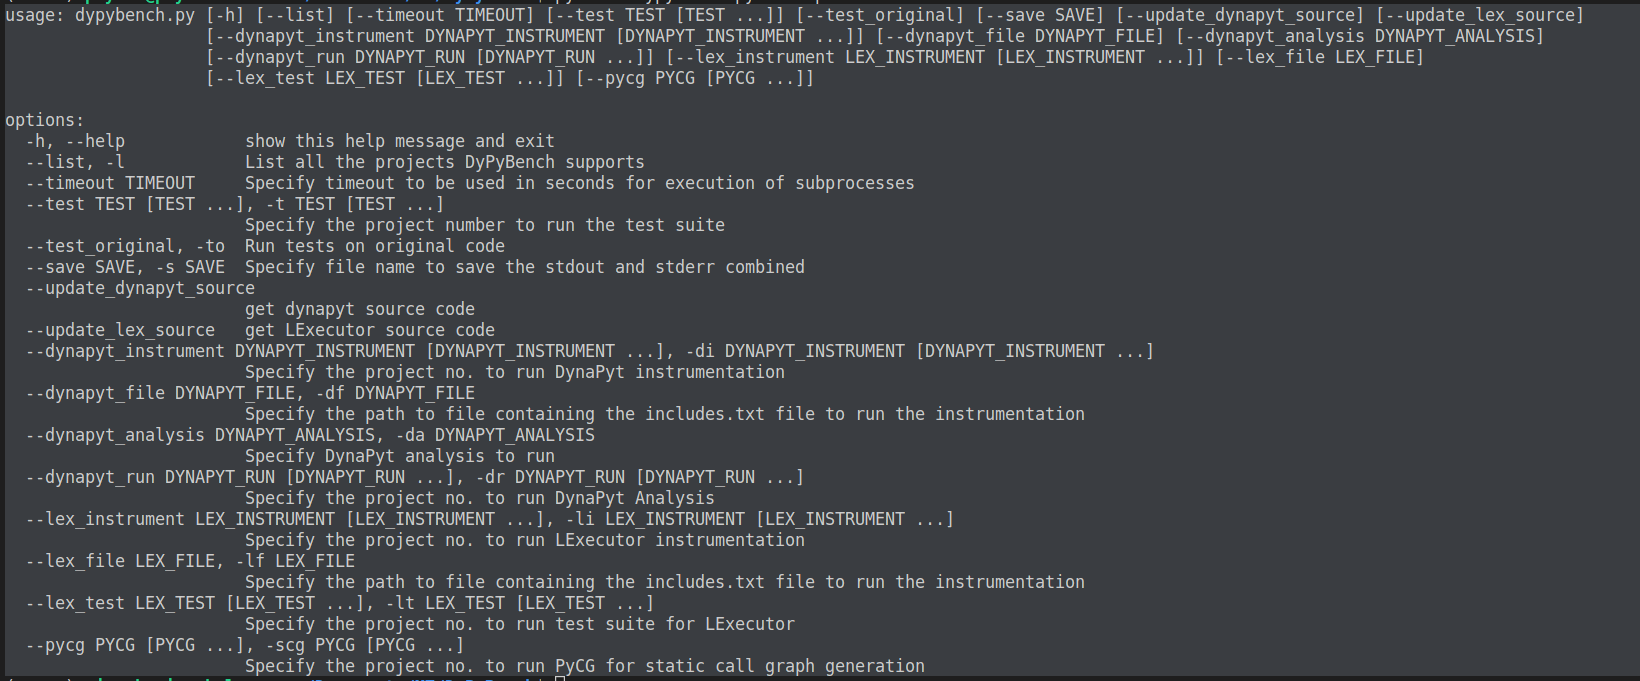
\includegraphics[width=1\linewidth]{figures/implementation/command-line-options.png}
    \caption[Command Line Options]{\label{fig:command-line-options}Command Line Options}
\end{figure}

\section{Integrating Code Analysis and Neural Network Tools}
\label{impl:Integrating Tools}
With the access interface to the benchmark, we integrate the neural network tool LExecutor and the code analysis tools PyCG and DynaPyt.
These tools need projects which do not have failed test cases in order to run efficiently.
However, the some of the projects that we installed in the benchmark have test cases that fail.
To handle this challenge, we skip the test cases which fail using a pytest marker.
In some cases we need to skip entire files, since all the test cases in the file fails.
The two types of pytest markers are as shown in the Listing \ref{code:pytest_marker}.
The marker shown on line 1 skips the entire file from execution, whereas line 3 shows the marker that skips only the test function.
\begin{lstlisting}[caption=Skip Test Case using Pytest Marker,label=code:pytest_marker,language=Python]
pytestmark = pytest.mark.skip("skip for dypybench")

@pytest.mark.skip("skip for dypybench")
\end{lstlisting}

We create a copy of the files for which we add pytest marks and replace the files in the original project directory using a Python script provided in the utility.
We also add this step of replacing files to the automation script of installation for future installations.

We use the source code of LExecutor and DynaPyt in our benchmark.
To access interface provides the arguments of \textit{\--\--udapte\_lex\_source} and \textit{\--\--update\_dynapyt\_source} to clone or update the source code of LExecutor and DynaPyt respectively from Git.
The following sections give more implementation details on the integration of LExecutor, PyCG and DynaPyt and the access interface arguments for them.

\subsection{LExecutor}
We clone the source code and create a Python virtual environment with the dependencies from the bash script when the argument \textit{\--\--update\_lex\_source} is run from the access interface.
Since LExecutor works in two steps to generate traces files, we provide two bash scripts one for each step.
The first script instruments the source code of the project and the second script generates trace files by executing the project.  
The instrumentation is not necessarily done on all the source files, but rather the files that run during execution.
In this work, we provide the files to be instrumented inside a text file as a list.
The text file contains a list of two space separated values, the first specifies the name of the project and the second specifies the path of the file to be instrumented.
We also provide a Python script to generate this text file, by parsing all the projects and filtering out the source files.
Certain files are excluded from this text file to avoid issues with running test suite.
However, this text file can be created by any means in the required format.
The Listing \ref{code:lex_instrument.txt} shows sample entries from the above mentioned text file.
This text file is specified to \textit{\--\--lex\_file} argument from the access interface.

\newpage
\begin{lstlisting}[caption=lex\_instrument\_all.txt,label=code:lex_instrument.txt,language=Bash]
grab ./temp/project1/tests/test_grab_pickle.py
grab ./temp/project1/tests/test_spider_queue.py
grab ./temp/project1/tests/test_ext_rex.py
grab ./temp/project1/tests/test_grab_cookies.py
errbot ./temp/project18/errbot/core_plugins/chatRoom.py
errbot ./temp/project18/errbot/core_plugins/backup.py
errbot ./temp/project18/errbot/core_plugins/acls.py
\end{lstlisting}

The argument \textit{\--\--lex\_instrument} triggers the first bash script to instrument the files specified in the above text file for the specified project.
This script executes the command shown in Listing \ref{code:lex_instrument}.
The parameter \$\{@:4\} is replaced by the space separated file paths. 
\begin{lstlisting}[caption=LExecutor Instrumentation,label=code:lex_instrument,language=Bash]
python -m lexecutor.Instrument --files ${@:4} --iids /DyPyBench/iids.json --validate
\end{lstlisting}

The second bash script mentioned above is triggered by the option \textit{\--\--lex\_test}, which simply runs the test suite of the specified project using command shown in Listing \ref{code:lex_test}.
The parameter \$3 is replaced by the test suite directory specified in github-url.txt.
\begin{lstlisting}[caption=LExecutor Test Suite Execution,label=code:lex_test,language=Bash]
pytest $3
\end{lstlisting}

The instrumentation also generates a iids.json file which is used by the LExecutor to convert the traces files into training data for the neural model.
We use the various utility functions provided in the benchmark for gathering trace files, inspecting the output of trace files and training logs of LExecutor.

\subsection{PyCG}
The argument \textit{\--\--pycg} from the access interface triggers the execution of a bash script which first installs the pycg package to the virtual environment of the specified project.
Then the script triggers the PyCG commands as shown in the Listing \ref{code:pycg}.
Only one of the two commands is executed based on the if condition shown on line 1, which checks if the test suite is a directory or a file.
The command on line 6 specifies all the .py files in the test suite directory as the entry point for the call graphs.
\begin{lstlisting}[caption=PyCG Execution,label=code:pycg,language=Bash]
if [[ $4 == "file" ]]
then
    pycg --package ./project$2 project$2/$3 -o pycg_$2.json
elif [[ $4 == "folder" ]]
then
    pycg --package ./project$2 $(find project$2/$3 -type f -name "*.py") -o pycg_$2.json
fi
\end{lstlisting}

As we can see from the Listing \ref{code:pycg}, the output file is generated for each project in the project folder.
Utility functions provided in the benchmark are used to collect these JSON output files for further analysis.  

\subsection{DynaPyt}
The argument \textit{\--\--update\_dynapyt\_source} from the access interface, executes a bash script to clone the source code of DynaPyt.
Similar to LExecutor, DynaPyt works in two steps,i.e., instrumentation and execution.
Each of these steps trigger separate bash scripts.
DynaPyt uses different modules to instrument directory and files.
We need to specify the files and folders which are to be instrumented.
Similar to LExecutor, we provide a text file which contains the list of directories and files which we want to instrument.
However, the format of the file is different compared to LExecutor.
This text file, has 3 space separated values on each line.
The first value is the project name, whereas the second value is the flag indicating file (f) or directory (d).
The third value in the space separated entry is the path of directory or file, relative to the root of the project.
Listing \ref{code:dynapyt_instrument.txt} shows some sample entries from this file.
This text file is specified to \textit{\--\--dynapyt\_file} argument from the access interface.
\begin{lstlisting}[caption=dynapyt\_instrument\_all.txt,label=code:dynapyt_instrument.txt,language=Bash]
flask-api d ./flask_api
schedule d ./schedule
schedule f ./test_schedule.py
Pillow d ./src
Pillow d ./Tests
supervisor d ./supervisor
streamparse d ./streamparse
\end{lstlisting}

In this work, we provide two such text files are provided for instrumentation, one which includes all the source files and the test files and the other which excludes test files.
To instrument the code, the first bash script first copies the DynaPyt source code that was cloned to the specific project directory.
Then, DynaPyt is installed with its dependencies into the virtual environment of the specific project.
Finally, the bash script runs the command to instrument the files or folder based on the flag provided by the above mentioned text file.
The instrumentation is based on the hooks provided by DynaPyt for the particular analysis.
Therefore, we need to provide the name of the analysis to be performed.
We provide this with the argument \textit{\--\--dynapyt\_analysis} to the access interface.
The two instrumentation commands are shown in the Listing \ref{code:dynapyt_instrument}. 

\newpage
\begin{lstlisting}[caption=DynaPyt Instrumentation,label=code:dynapyt_instrument,language=Bash]
if [[ $5 == "d" ]]
then
    #run instrumentation on the given directory
    python -m dynapyt.run_instrumentation --directory $3 --analysis $4
elif [[ $5 == "f" ]]
then
    #run instrumentation on the given file
    python -m dynapyt.instrument.instrument --files $3 --analysis $4
fi
\end{lstlisting}

The execution of test suite to perform the dynamic analysis is done using another bash script.
This script, first create an entry file to run all the tests using pytest module with the parameter import-mode set to importlib.
The Listing \ref{code:run_all_test.py} shows a sample of the entry file created above.
We then trigger the execution of tests with \textit{run\_analysis} module provided by dynapyt, specifiying the above entry file and the name of the analysis.
Listing \ref{code:dynapyt_test} shows the creation of the entry file on line 1 and execution with run\_analysis on line 3.
\begin{lstlisting}[caption=DynaPyt Execution Entry File,label=code:run_all_test.py,language=Python]
import pytest

pytest.main(['--import-mode=importlib','/home/piyush/Documents/MT/CallGraph/flask-api/flask_api/tests/'])
\end{lstlisting}
\begin{lstlisting}[caption=DynaPyt Test Suite Execution,label=code:dynapyt_test,language=Bash]
printf "import pytest\n\npytest.main(['--import-mode=importlib', '$ROOT_DIR/temp/project$2/$4'])\n" > run_all_tests.py

python -m dynapyt.run_analysis --entry ./run_all_tests.py --analysis $3
\end{lstlisting}

\section{Call Graph Analysis}
\label{impl:Call Graph Analysis}
In this work, we developed a new analysis in DynaPyt to generate call graphs during run-time.
This analysis is named CallGraph and we use the output of this analysis for comparison with PyCG.
We use the function pre\_call hook provided by DynaPyt and create the call graph in the form of dictionary.
A key in this dictionary is the fully qualified names of the caller method and the value for this key is a list of fully qualified names of called methods.
At the end of the execution, i.e., after the all the test cases are run we output the dictionary to a JSON file.
A Python utility script provide by the benchmark collects all the JSON files from the projects that were dynamically analyzed.
Listing \ref{code:pre_call_hook} shows the code of the pre\_call hook implemented for the analysis.
The complete code for the analysis is shown in the Listing \ref{code:CallGraphAnalysis}.

\newpage
\begin{lstlisting}[caption=Function Pre-Call Hook in Call Graph Analysis,label=code:pre_call_hook,language=Python,linerange={19-53}]
from typing import Callable, Tuple, Dict
import logging
import libcst as cst
import libcst.matchers as m
from .BaseAnalysis import BaseAnalysis
from ..utils.nodeLocator import get_parent_by_type
import json
from inspect import getmodule

class CallGraph(BaseAnalysis):
    def __init__(self):
        super(CallGraph, self).__init__()
        logging.basicConfig(filename="dynapyt.json", format='%(message)s', level=logging.INFO)
        self.graph = {}

    '''
    DynaPyt hook for pre function call
    '''
    def pre_call(self, dyn_ast: str, iid: int, function: Callable, pos_args: Tuple, kw_args: Dict):
        ast, iids = self._get_ast(dyn_ast)
        module = getmodule(function)
        module = str(module).split(' ')[1] if module is not None else "''"
        # calling function 
        caller = get_parent_by_type(ast, iids.iid_to_location[iid], m.FunctionDef())
        # called function
        if hasattr(function, "__qualname__"):
            callee = module[1:-1] + '.' + function.__qualname__ if module != "''" else function.__qualname__
        else:
            temp = str(function)
            callee = temp
        
        #file name
        key = dyn_ast.replace('.py.orig', '').replace('/','.')
        
        if caller is None:
            f = key
        else:
            # if caller is a part of class, find the class name
            caller_parent = get_parent_by_type(ast, iids.iid_to_location[iid], m.ClassDef())
            if caller_parent is None:
                f = key + '.' + caller.name.value
            else:
                f = key + '.' + caller_parent.name.value + '.' + caller.name.value

        # if caller already added
        if f in self.graph.keys():
            temp = self.graph[f]
            # filter dupilcate callees
            if callee not in temp:
                temp.append(callee)
                self.graph[f] = temp
        else:
            self.graph[f] = [callee]
    
    def end_execution(self):
        try:
            logging.info(json.dumps(self.graph))
        except Exception:
            logging.info("{")
            for idx, key in enumerate(self.graph):                
                if not idx == (len(self.graph.keys()) - 1):
                    logging.info("{} : {}, ".format(key, self.graph[key]))
                else:
                    logging.info("{} : {}".format(key, self.graph[key]))
            logging.info("}")
                
\end{lstlisting}
